\documentclass[a4paper]{ctexbook}
\usepackage[margin=1in]{geometry}
\usepackage{amsmath}
\usepackage{amsthm} % proof
\usepackage{amssymb} % \mathbb
% \usepackage{amstext} % \text
\newtheorem{theorem}{定理}[chapter] %定理按章编号
\newtheorem{lemma}{引理}[chapter]
\newtheorem{property}{性质}[chapter]
\newtheorem{example}{例}[chapter]
\usepackage{listings}
\lstset{language=C++, basicstyle=\ttfamily, frame=lines}
\newcommand{\idx}{\mathrm{idx}}

\begin{document}
  \chapter{图论高级算法}
  \section{最大流}
  最大流算法分成两大类:增广路(augmengting path)算法与预流推进(preflow-push)算法。
  这一节介绍的三个算法,都属于增广路算法。
  下面给出几个术语和定义。
  \subsubsection*{流网络}\label{notations}
  最大流问题(maximum flow problem)是网络流问题(network flow problem)的一种。网络流问题的研究对象是流网络(flow network),在某些文献中流网络也称作网络流图(network flow graph)。流网络$G=(V,E,c,s,t)$是一个有向图,$V$、$E$是其点集与边集,点和边的数目分别记作$n$、$m$。$c\colon V\times V\to \mathbb{N}$是边的容量函数,每条边$(u,v)\in E$都有一容量$c(u,v)\in \mathbb{N}$,若$(u,v)\notin E$则$c(u,v) = 0$。$s$和$t$是流网络中的两个特殊点,分别称作源点和汇点。为简便计,流网络简称「网络」或「图」,简记作$G=(V,E)$。

  自环在网络中无意义,我们规定图$G$中不含自环。%允许网络中有重边。
  下文在论述、证明关于网络流的原理、性质或定理时,为了表示上的方便,我们对流网络做出两条限定:
  \begin{enumerate}
    \item 图中不存在重边;\label{Restrict:1}
    \item 图中不存在反向边,即若$(u,v)\in E$,则$(v,u)\notin E$。\label{Restrict:2}
  \end{enumerate}
  这两条限定都不妨碍一般性。我们可以通过将容量相加把重边合为一条边,反向边可以通过新增一个节点来消除。请读者注意,上文所谓「表示上的方便」是指一条边可以通过两个端点唯一确定。下文我们要介绍的算法和代码可以处理含有重边或反向边的图,这两条限定都不是根本性的,仅仅是为了方便表述而已。

  \subsubsection*{流}
  流是满足下述两个性质的实值函数$f\colon V\times V\to\mathbb{R}$:
  \begin{description}
    \item[容量限制:]对任意$u,v \in V$,有 $0\le f(u,v)\le c(u,v)$。
    \item[流守恒:]对任意$u\in V-\{s,t\}$,有$\sum\limits_{v\in V}f(v,u)= \sum\limits_{v\in V}f(u,v)$
  \end{description}
  $f(u,v)$即边$(u,v)$上的流量,若$(u,v)\notin E$,$f(u,v) = 0$。
  从源点$s$到汇点$t$的总流量称作流$f$的值,记作$|f|$,不难得出
  $$|f| = \sum_{v\in V}f(s,v) - \sum_{v\in V}f(v,s)\text{,}$$
  最大流问题即在给定的网络$G$中求一个值最大的流。

  \subsection{增广路方法}
  增广路方法是求解最大流问题的一种方法。本章要介绍的三个最大流算法都是基于增广路方法的。增广路算法涉及三个重要概念:残量网络,增广路,割。
  \subsubsection*{残量网络}
  给定流网络$G=(V,E,c,s,t)$和$G$上的一个流$f$。残量网络$G_f=(V,E_f,c_f, s, t)$是由$G$和$f$所导出的一个网络,简记作$G_f=(V,E_f)$。首先定义残余容量$c_f$:
  \[
  c_f(u,v) =
  \begin{cases}
    c(u,v) - f(u,v) & \text{若$(u,v)\in E$,}\\
    f(v,u) & \text{若$(v,u)\in E$,} \\
    0 & \text{其他情况.}
  \end{cases}
  \]
  这里需要指出我们提出限制\ref{Restrict:2} 的用意。$(u,v)\in E$和$(v,u)\in E$同时成立会给$c_f$的定义带来形式上的不便。残量网络$G_f$的边集$E_f$定义为
  \[
  E_f = \{(u,v)\in V\times V\colon c_f(u,v)>0\}.
  \]
  除了可能含有反向边,残量网络也符合流网络的定义;而我们已经指出「不含反向边」并非根本性的要求,借助残余容量$c_f$,我们可以类似地定义残量网络上的流,称作\emph{残量流}。

  我们考虑残量流的原因在于,借助残量网络$G_f$上的残量流$f'$,可以将网络$G$上的流$f$修改成一个值更大的流$f\uparrow f'$;即用$f'$ 增广 $f$,这正是「增广」二字含义所在。增广方法为:
  \[
  (f\uparrow f')(u,v) =\begin{cases}
  f(u,v) + f'(u,v) - f'(v,u) & \text{若$(u,v)\in E$,} \\
  0 & \text{其他情况.}
\end{cases}
  \]
  不难证明$|f\uparrow f'| = |f| + |f'|$。
  \subsubsection{增广路}
  增广路是残量网络$G_f$上从$s$到$t$的一条简单路径。有了增广路$p$,很容易得到一个残量流$f_p$。
  \[
  f_p(u,v) =\begin{cases}
  c_f(p) & \text{若边$(u,v)$在路径 $p$ 上,}\\
  0 & \text{其他情况.}
\end{cases}
  \]
  其中$c_f(p) = \min\{c_f(u,v)\colon (u,v)\text{ 在路径 }p\text{ 上} \}$,$c_f(p)$称作路径$p$的残余容量。易见,$|f_p| = c_f(p) > 0$。

  增广路方法即,从图$G$上的某个初始流$f$(比如零流)开始,在$G_f$找一条增广路$p$;沿着$p$增广,更新$f$和$G_f$;如此循环,直到$G_f$上找不到增广路。此时$f$便是$G$上的一个最大流。下面要介绍的最大流最小割定理证明了增广路方法的正确性。
  \subsubsection*{流网络的割}
  为了给出最大流最小割定理,我们先介绍割的概念。
  将流网络$G=(V,E)$的点集$V$划分成两个子集$S$和$T=V-S$使得$s\in S$且$t\in T$,$(S,T)$称作$G$的一个割。令$f$为$G$上的一个流,割$(S,T)$之间的\emph{净流}$f(S,T)$定义为
  \[
  f(S,T) = \sum_{u\in S}\sum_{v\in T}f(u,v) - \sum_{u\in S}\sum_{v\in T}f(v,u)
  \]
  不难证明,对$G$的任意一个割$(S,T)$都有$f(S,T) = |f|$。
  割$(S,T)$的容量$c(S,T)$定义为
  \[
  c(S,T) = \sum_{u\in S}\sum_{v\in T}c(u,v)
  \]
  网络的最小割即所有割之中容量最小者。显然,对于$G$上的任意一个流$f$和$G$的任意一个割$(S,T)$都有 $f \le c(S,T)$。
  \begin{theorem}[最大流最小割定理]
    若$f$是流网络$G=(V,E,c,s,t)$上的一个流,则下列三个命题等价:
    \begin{enumerate}
      \item $f$是$G$上的一个最大流。
      \item 残量网络 $G_f$ 上无增广路。
      \item 存在某个割$(S,T)$满足$|f| = c(S,T)$。
    \end{enumerate}
  \end{theorem}
  \begin{proof}
    (1)$\Rightarrow$(2):显然。

    (2)$\Rightarrow$(3):假设$G_f$中无增广路,即$G_f$上不存在$s\leadsto t$路径。令$S=\{v\in V\colon G_f\ \text{上有}\ s\leadsto v\ \text{路径}\}$,$T=V-S$,易见$t\notin S$,故$(S,T)$是一个割。考虑两点$u\in S$和$v\in T$。若$(u,v)\in E$,则必有$f(u,v)=c(u,v)$;因为若不然则有$(u,v)\in E_f$,即$v\in S$。若$(v,u)\in E$,则必有$f(v,u)=0$;因为若不然则有$c_f(u,v) = f(v,u) > 0$,即$(u,v)\in E_f$,仍有$v \in S$。若$(u,v)\notin E$且$(v,u)\notin E$,则$f(u,v)=f(v,u)=0$。因此我们有
    \begin{align*}
        f(S,T) &= \sum_{u\in S}\sum_{v\in T}f(u,v) - \sum_{v\in T}\sum_{u\in S}f(v,u)\\
        &= \sum_{u\in S}\sum_{v\in T}c(u,v) - \sum_{v\in T}\sum_{u\in S}0\\
        &= c(S, T)
    \end{align*}
    所以 $|f| = f(S,T) = c(S, T)$。

    (3)$\Rightarrow$(1):由于对任意割$(S,T)$都有$|f|\le c(S,T)$,故$|f|=c(S,T)$蕴含着$f$是一个最大流。
  \end{proof}

  不难看出,高效地实现增广路方法应从两个方面考虑:
  \begin{enumerate}
    \item 如何快速地在残量网络$G_f$上找一条增广路。\label{Approach:1}
    \item 如何减少增广的次数。\label{Approach:2}
  \end{enumerate}
  我们已经知道,通过深度优先搜索(DFS)或宽度优先搜索(BFS)可在线性间内找到一条增广路。
  在下一小节中我们将证明,如果每次都沿着\emph{最短增广路}(shortest augmenting path,SAP)增广,那么增广次数是$O(VE)$的。沿着最短增广路增广的算法统称为最短增广路算法。下面三个小节中要介绍的算法都属于最短增广路算法。
  \subsection{Edmonds-Karp算法}
  Edmonds-Karp是SAP算法的朴素实现。代码如下:
  \lstinputlisting{code/ek.cpp}
  说明:
  \begin{enumerate}
    \item 用链式前向星存图。
    \item 对任意边$e \in E$,$e$在边数组中的下标$\idx(e)$为偶数,$e$的反向边$e'$的下标$\idx(e') = \idx(e) + 1$。
  \end{enumerate}

  下面我们来分析Edmonds-Karp算法的时间复杂度。用$\delta_f(u,v)$表示残量网络$G_f$上从$u$到$v$的距离,$G_f$中边的长度都是$1$。
  \begin{lemma}\label{Lemma:1}
      用Edmonds-Karp算法求流网络$G=(V,E,c,s,t)$的最大流的过程中,对任意节点$v\in V-\{s,t\}$,残量网络$G_f$上从源点$s$到$v$的距离$\delta_f(s,v)$在每次增广之后不会减小。
  \end{lemma}
  \begin{proof}
      假设此命题不成立。
      设$v$是$V-\{s,t\}$中一点;令$f$为「$s$到$v$的距离减小」首次出现之前的流,令$f'$为$f$增广之后的流。再令$v$为满足$\delta_f(s,v)>\delta_{f'}(s,v)$的点中$\delta_{f'}(s,v)$最小的一个点。令$p = s \leadsto u\to v$为$G_{f'}$中从$s$到$v$的一条最短路,因而有$(u,v)\in E_{f'}$且
      \begin{equation}
          \delta_{f'}(s,u) = \delta_{f'}(s,v) - 1 . \label{Eq:1}
      \end{equation}
      又由于$v$是满足$\delta_f(s,v)>\delta_{f'}(s,v)$的点中$\delta_{f'}(s,v)$最小者,我们有
      \begin{equation}
          \delta_{f'}(s,u)\ge\delta_f(s,u). \label{Ineq:1}
      \end{equation}
      由上两式我们能推导出$(u,v)\notin E_f$。若不然,即$(u,v)\in E_f$,则有
      \begin{align*}
          \delta_f(s,v) &\le \delta_f(s,u)+1 &\text{依据三角形不等式} \\
          &\le \delta_{f'}(s,u) + 1 &\text{依据 \eqref{Ineq:1} 式}\\
          &= \delta_{f'}(s,v) &\text{依据 \eqref{Eq:1} 式}
      \end{align*}
      这与$\delta_{f'}(s,v) < \delta_f(s,v)$矛盾。

      由$(u,v)\notin E_f$且$(u,v)\in E_{f'}$,我们可以推知在$G_f$上所选的那条增广路一定经过了边$(v,u)$。因此有
      \begin{align*}
          \delta_f(s,v) &= \delta_f(s,u) - 1  \\
          &\le\delta_{f'}(s,u) - 1 & \text{(根据 \eqref{Ineq:1} 式)}\\
          &=\delta_{f'}(s,v) - 2 & \text{(根据 \eqref{Eq:1} 式)}
      \end{align*}
      这与我们的假设$\delta_{f'}(s,v) < \delta_f(s,v)$相矛盾。
  \end{proof}

  \begin{theorem}\label{T:number-of-augmentations}
      在流网络$G=(V,E,c,s,t)$上,Edmonds-Karp算法的总增广次数为$O(VE)$。
  \end{theorem}
  \begin{proof}
      设$p$为残量网络$G_f$中的一条增广路,$(u,v)$为$p$上的一条边。若有$c_f(p) = c_f(u,v)$,则称$(u,v)$为$p$的瓶颈边。不难看出,(i)沿着$p$增广后,$p$上的瓶颈边都消失了;(ii) $p$上至少有一条瓶颈边。下面我们证明:一条边在$G_f$上成为瓶颈边的次数至多为$|V|/2$。

      令$(u,v)$为残量网络$G_f$中的一条边。当$(u,v)$首次成为瓶颈边时,我们有
      \[
      \delta_f(s,v) = \delta_f(s,u) + 1 .
      \]
      增广之后,边$(u,v)$将从残余网络中消失。下一次$(u,v)$出现在残量网络中,必然是在某次$(v,u)$出现在增广路上之后。设上述「$(v,u)$成为增广路上的边」这一情况发生时$G$上的流为$f'$,则有
      \[
      \delta_{f'}(s,u) = \delta_{f'}(s,v) + 1.
      \]
      根据引理 \ref{Lemma:1} 有 $\delta_f(s,v)\le\delta_{f'}(s,v)$,因而有
      \begin{align*}
          \delta_{f'}(s,u) &= \delta_{f'}(s,v) + 1 \\
          &\ge \delta_f(s,v) + 1 \\
          &= \delta_f(s,u) + 2 .
      \end{align*}

      所以从某次$(u,v)$成为瓶颈边到$(u,v)$下一次成为瓶颈边,从源点$s$到$u$的距离至少增加$2$。初始时$s$到$u$的距离至少为$0$。从$s$到$u$的最短路上的中间节点必定不包含$s$,$u$ 或者$t$(边$(u,v)$在最短路上蕴含着$u\ne t$)。因此,只要$s\leadsto u$的路径存在,$s$到$u$的距离至多为$|V|-2$。所以在$(u,v)$首次成为瓶颈边之后,它最多还能在成为$(|V|-2)/2=|V|/2-1$次瓶颈边,共计$|V|/2$次。又由于在残量网络上有$O(E)$对点之间可能有边相连,在Edmonds-Karp算法运行过程中瓶颈边的总数是$O(VE)$的。
  \end{proof}

  我们可以通过BFS在$O(E)$的时间内在残量网络上找到一条$s\leadsto t$最短路,因此Edmonds-Karp算法的时间复杂度为$O(VE^2)$。严格说来,BFS的时间复杂度应为$O(V+E)$;但是在流网络$G$中一个点应至少有一条边与其相连(孤立的点是无意义的)所以我们有$|V|\le2|E|$。
  \subsection{Dinic算法}
  \lstinputlisting{code/dinic.cpp}
  Dinic算法是对Edmonds-Karp算法的改进,它的时间复杂度是$O(n^2m)$\footnote{在\S\ref{notations} 中,我们约定了$n=|V|$,$m=|E|$。}。下面给出Dinic算法的的代码,其中图的表示部分与Edmonds-Karp算法的代码相同,故略去。

  先介绍Dinic算法用到的两个概念:分层图(level graph)和阻塞流(blocking flow)。
  \subsubsection*{分层图}
  设$f$是网络$G$上的一个流,以$s$为起点对$G_f$做一次BFS,将$s$到$u$的距离记作$\mathrm{level}(u)$。$G_f$的分层图$G'_f$是由$G_f$所导出的一个流网络。$G'_f$定义为
  \[
  G'_f =(V, E'_f, c'_f, s, t)
  \]
  其中
  \begin{align*}
      E'_f &= \{(u,v)\in E_f\colon \mathrm{level}(v) = \mathrm{level}(u)+1\} \\
      c'_f(u,v) &=\begin{cases}
      c_f(u,v), & (u,v)\in E'_f;\\
      0, & (u,v)\notin E'_f.\end{cases}
  \end{align*}
  简记作$G'_f =(V, E'_f)$。
  \subsubsection{阻塞流}
  首先要指出的是,由$G_f$所导出的分层图$G'_f$完全符合\S\ref{notations} 中流网络的定义($G'_f$与$G_f$不同的地方在于$G'_f$中一定不含有反向边)。此外,不难看出$G'_f$中的任意一条$s\leadsto t$路径都是$s\leadsto t$最短路。

  设$f$是网络$G=(V,E)$上的一个流,$(u,v)\in E$是$G$上的一条边;若$f(u,v) = c(u,v)$则称边$(u,v)$是\emph{饱和}的。又设$f'$是分层图$G'_f$上的一个流,若$G'_f$中的任意一条$s\leadsto t$路径上都至少有一条饱和边,则称$f'$是$G'_f$上的一个阻塞流。注意,$G'_f$上阻塞流未必是$G'_f$上的最大流,图\ref{Fig:blocking-flow} 就是一个例子。
  \begin{figure}
      \centering
      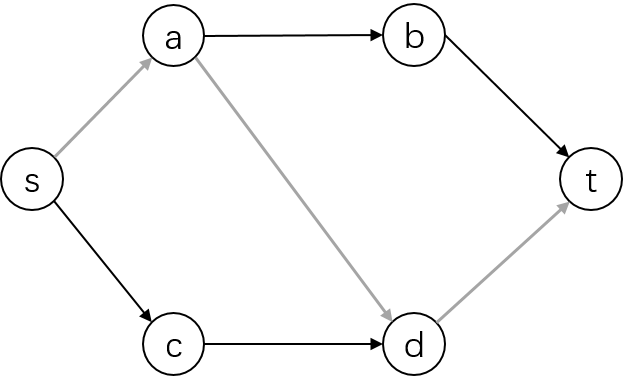
\includegraphics[scale=0.5]{figures/blocking-flow.png}
      \caption{阻塞流非最大流的一个例子。黑色边是非饱和边,灰色边是饱和边}
      \label{Fig:blocking-flow}
  \end{figure}

  下面考虑如何构造阻塞流。前面已经提到,分层图$G'_f$是一个流网络;所以一个自然的想法便是在$G'_f$上不断地DFS寻找增广路\footnote{准确地说应该是「在$G'_f$的残量网络上找增广路」,但我们在$G'_f$要求的是一个阻塞流而不是最大流,无须考虑反向边。}并沿着找到的增广路增广。每次增广至少会使一条边饱和,所以至多增广$m$次;可以在$O(m)$的时间内在分层图上找到一条$s\leadsto t$增广路。,所以构造阻塞流的复杂度不超过$O(m^2)$。下面我们介绍一种称作「当前边」的优化\footnote{有的资料将此优化称作当前弧优化},可使构造阻塞流的复杂度达到$O(nm)$。另外还有一个称作「多路增广」的实现技巧,可进一步优化时间复杂度。
  \subsubsection*{当前边优化}
  对分层图中的每个节点$u$维护一个当前边,初始时初始时$u$的当前边为$u$的邻接边表中的第一条边。每次DFS到点$u$时,从$u$的当前边,设为$(u,v)$,向下递归。若DFS($v$)未找到从$v$到汇点$t$ 的路径,就把$u$的当前边变为$u$的邻接边表中的下一条边,这相当于将边$(u,v)$从分层图中删除;若找到了到$t$的路径就一路回溯。

  我们来分析这种方法构造阻塞流的复杂度。整个过程的复杂度可以化归为调用DFS($v$)的次数。若DFS($v$)的返回值为「找到了路径」则这种调用以$l$个为一组($l$为分层图的层数),每次找到一条$s\leadsto t$路径至少使一条边饱和,这种调用至多有$lm\le nm$次\footnote{残量网络$G_f$中最多有$2m$条边,但是边$(u,v)$和边$(v,u)$不可能同时出现在分层图$G'_f$中,所以$G'_f$中至多有$m$条边。}。若DFS($v$)的返回值为「未找到路径」则有一条边被删除,故这种调用不超过$m$次。所以构造阻塞流的复杂度为$O(nm)$。
  \subsubsection*{多路增广}
  用$c_f(v)$表示DFS到$v$点时从$s$到$v$所经过的边的残余容量的最小值,$c_f(s) = \infty$。
  多路增广是指DFS到$t$点后不一直向上回溯到源点$s$,而是一旦回溯到$c_f(v)>0$的点$v$就从$v$继续向下递归。这里所说的「一旦回溯到$c_f(v)>0$的点$v$」也就是找到的$s\leadsto t$增广路上距离$s$点最近的\emph{饱和边}的起点。把$c_f(v)$也作为DFS的参数,即调用DFS($v$, $c_f(v)$)。当$c_f(v)$变为$0$时就终止DFS($v$, $c_f(v)$)过程。

  \subsubsection*{小结}
  借助分层图这一概念,我们可以很直观地理解引理 \ref{Lemma:1}。Dinic算法的过程就是不断的构造阻塞流,并用阻塞流来增广原来的流$f$;不难看出每次用阻塞流增广$f$之后,残量网络上的最短$s\leadsto t$路径的长度严格递增,所以Dinic算法最多构造$n-1$次阻塞流,因而复杂度为$O(n^2m)$。此复杂度上界是比较松的,Dinic算法的速度能满足大部分实际问题的要求。

  %(由于$G'_f$是$G_f$的子图,将$G'_f$上$s\leadsto t$路径称作增广路是不失严格性的)

  \subsection{ISAP算法}
  ISAP是Improved Shortest Augmenting Path的缩写,ISAP算法来源于R.K. Ahuja,T.L. Magnanti和J.B. Orlin三人合著的\emph{Network Flows: Theory, Algorithms, and Applications}一书的\S 7.4 shortest augmenting path algorithm中提到的对SAP算法的一个优化。我们先介绍SAP算法,然后再介绍此优化方法。顾名思义,ISAP算法也是一种最短增广路算法;ISAP算法中引入了一些新概念,下面一一介绍。
  \subsubsection*{距离标号}
  设$G(V,E,c,s,t)$是一个流网络,$f$是$G$上的一个流。在残量网络$G_f=(V,E_f)$上,我们定义一个距离函数$d\colon V\to\mathbb{N}$。若函数$d$满足下面两个条件,则称$d$为合法的距离函数:
  \begin{enumerate}
      \item $d(t) = 0$;
      \item $\forall (u,v)\in E_f, d(u) \le d(v) +1$.
  \end{enumerate}
  我们把$d(u)$称作节点$u$的\emph{距离标号},上述两条件称作合法条件。
  \begin{property}\label{P:lower_bound}
      若距离函数$d$合法,则距离标号$d(u)$是残量网络$G_f$上从$u$到$t$的距离的一个下界。
  \end{property}
  令$v=v_0\to v_1 \to\dots\to v_{k-1}\to v_k$为$G_f$上任意一条从$v$到$t$的长为$k$的路径。合法条件蕴含着
  \begin{align*}
      d(v_{k-1})&\le d(v_k)+1 = d(t)+1=1,\\
      d(v_{k-2})&\le d(v_{k-1})+1\le 2,\\
       &\vdots\\
      d(v) = d(v_0)&\le d(v_1) + 1 \le k.
  \end{align*}
  \begin{property}
      若$d(s)\ge n$则残余网络$G_f$中没有从源点$s$到汇点$t$的路径。
  \end{property}
  由于$d(s)$是$G_f$上从$s$到$t$的距离的一个下界,又$\delta_f(s,t)\le n-1$,所以$d(s)\ge n$意味着$G_f$上不存在$s\leadsto t$路径。

  若对每个点$u\in V$都有$\delta_f(u,t)=d(u)$,则称距离标记是准确的。
  \subsubsection*{允许边和允许路径}
  若边$(u,v)\in E_f$满足$d(u)=d(v)+1$则称$(u,v)$为\emph{允许边},否则称为非允许边。若$G_f$的一条$s\leadsto t$路径$p$完全由可行边构成,则称$p$为\emph{允许路径}。显然有
  \begin{property}
    可行路径是一条最短增广路。
  \end{property}

  \subsubsection*{SAP算法}
  SAP算法的思想与Dinic算法类似\footnote{这里所谓「类似」是指level($u$)与$d(u)$的意义有相似之处;但仍应注意分层图$G'_f$上的边和残余网络$G_f$中的可行边这两个概念的区别:若令$d(u)=\mathrm{level}(u)$,则分层图上的边一定是可行边;反过来不成立。}。确定一个初始的合法距离标号,SAP算法重复「DFS找可行路径」的过程,直到残量网络上不存在$s\leadsto t$路径。DFS由前进(advance)、后退(retreat)和重标号(relabel)三种操作构成,详述如下:

  从$s$开始,沿着允许边走,试图到达$t$;若能到达$t$,则沿着找到的最短增广路增广,在新的残量网络上继续寻找允许路径。与Dinic算法不同的是,若走到$u$点之后无法继续\emph{前进},即没有以$u$为起点的可行边,则增大$u$的距离标号,将$d(u)$更新为$\min\{d(v)+1\colon (u,v)\in E_f\}$,这一操作称作\emph{重标号};然后\emph{后退}一步继续寻找可行边。上述DFS过程采用递归实现比较方便,但顾及效率,下面我们给出SAP算法的迭代实现。在迭代实现中,我们需要维护(i)每个点的「当前边」,点$u$的当前边是指走到$u$时要选择的那条出边;(ii)当前找到的「部分可行路径」。
  \lstinputlisting{code/sap.cpp}
  %DFS走过一条允许边称作\emph{前进}(advance);回溯一步称作\emph{回退}(retreat)。
  \subsubsection{SAP算法的正确性}
  不难验证:(i)重标号操作使一个点的距离标号严格增大;(ii)增广和重标号这两种操作能维持距离标号的合法性。再结合性质\ref{P:lower_bound},可以推出:(i) SAP算法能在有限次重标号操作之后找到一条最短增广路;(ii) SAP算法能在有限次重标号和增广之后求出一个最大流。
  %要证明SAP算法的正确性只要证明增广和重标号这两种操作能保证距离标号的合法性。首先,不难看出重标号操作使一个点的距离标号严格增大。先考虑增广操作,设边$(u,v)$在SAP算法找到的某条增广路上,若$(v,u)$是增广之后新出现在残量网络上的边,$d(u)\le d(v)+1$蕴含着$d(v)\le d(u)+1$。再考虑重标号操作,我们只要证明在重标号操作修改了$d(u)$之后,$u$的所有入边仍是允许边($u$的所有出边在重标号之后显然仍满足合法条件)。
  \subsubsection{SAP算法的复杂度}
  SAP算法的复杂度可分成四部分考虑:
  \begin{enumerate}
    \item 检查点的出边是否为允许边
    \item 重标号
    \item 前进和后退的总次数
    \item 增广
  \end{enumerate}

  注意到(i)对点$u$重标号的前提是遍历$u$的出边而未找到允许边;(ii)对$u$重标号的复杂度即遍历$u$的出边的复杂度。所以重标号的总复杂度不超过检查点的出边是否为允许边的复杂度。我们可以得出
  \begin{property}
    若SAP算法对每个点重标号不超过$k$次,则「检查点的出边是否为允许边」和「计算新距离标号」的总复杂度为$O(k\sum\limits_{u\in V}|E(u)|)=O(km)$。其中$E(u)=\{(v,w)\in E\colon v= u \text{ 或}\ w = u\}$。
  \end{property}
  另外注意到,每次对点$u$重标号之前我们已经找到了一条完全由允许边组成的$s\leadsto u$路径,从而有$d(u)\le d(s)< n$;又重标号之后$d(u)$至少增加$1$,所以$u$经历过至多$n$次重标号。因此(i)重标号的总次数为$O(n^2)$,后退的总次数也是$O(n^2)$;(ii)寻找允许边和计算新距离标号的总复杂度为$O(nm)$。

  再考虑增广的总复杂度。采用定理\ref{T:number-of-augmentations} 的证明思路,我们可以证明:
  \begin{theorem}
    SAP算法的增广次数为$O(nm)$。
  \end{theorem}
  因为一次增广的复杂度为$O(n)$,故增广的总复杂度为$O(n^2m)$,从而前进的总次数为$O(n^2m+n^2)=O(n^2m)$。综上所述,SAP算法的复杂度为$O(n^2m)$。
  \subsubsection{优化}
  SAP算法终止的条件是$d(s)\ge n$,但实际中往往在$d(s)\ge n$达成之前很久就已经算出一个最大流了。在最大流求出之后进行的种种操作显然是多余的,下面我们要介绍的优化能及时检测到当前残量网络上出现了一个最小割亦即求得了一个最大流。

  维护一个长为$n$的数组num,num[$i$]表示当前残量网络上距离标号为$i$的点的数目($0\le i < n$)。初始的合法距离标号不能任意设置,需要保证num数组中的非零项连续,亦即存在某个下标$l$使得$\mathrm{num}[0],\mathrm{num}[1],\dots,\mathrm{num}[l]$都大于零,数组中其他项都为零。要满足这一条件至少有两个选择:(i)所有距离标号都置为$0$;(ii)从$t$点开始反向BFS,求出准确距离标号。每次将某点的距离标号从$k_1$提高到$k_2$,num[$k_1$]减一,num[$k_2$]加一;若num[$k_1$]变为零则终止算法。

  下面来证明此优化的正确性。设num[$k_1$]减为零时求得的流为$f$。令$S=\{v\in V\colon d(v)>k_1\}$,$T=\bar{S}=\{v\in V\colon d(v)<k_1\}$;不难验证$s\in S$,$t\in T$;即$(S,T)$是流网络$G=(V,E)$的一个割。我们将证明$|f|=c(S,T)$。考虑点对$u\in S$和$v\in T$,由$S$和$T$的定义可知$d(u)>d(v)+1$,所以$(u,v)\notin E_f$。由$(u,v)\notin E_f$可推出(i)若$(u,v)\in E$则必有$f(u,v) = c(u,v)$;(ii)若$(v,u)\in E$则必有$f(v,u)=0$。因此我们有
  \begin{align*}
    f(S,T) &= \sum_{u\in S}\sum_{v\in T}f(u,v)-\sum_{v\in T}\sum_{u\in S}f(v,u)\\
    &= \sum_{u\in S}\sum_{v\in T}c(u,v)-\sum_{v\in T}\sum_{u\in S}0\\
    &= c(S,T)
  \end{align*}
  所以$|f|=f(S,T)=c(S,T)$。

  下面给出ISAP算法的代码,我们采用逆向BFS求每个点的准确距离标号,其中\texttt{augment}函数与SAP算法中相同,略去。
  \lstinputlisting{code/isap.cpp}
  \subsection{网络流的建图}
  网络流问题包括最大流的费用流两大类,这一小节我们只考虑最大流的建图(或称建模)。最大流的建图一般从流和隔两方面考虑,
  \section{费用流}
  \section{二分图}
  \subsection{最大流和二分图}
  \subsection{匈牙利算法}
  \subsection{二分图模型应用}
  \section{图的连通}
  \subsection{强连通-Tarjan算法}
  \subsection{双连通}
  \subsection{2-SAT问题}
  \chapter{A DUMMY CHAPTER}
\end{document}
